\chapter{Specific Requirements}

\section{External Interface Requirements}

\subsection{User Interfaces}

\subsection{Hardware Interfaces}
DREAM is a web application, as such each user should own a device capable of installing a modern browser. Form factor of the device doesn't matter, as DREAM application is fully responsive.

\subsection{Software Interfaces}
A modern browser is necessary to use the system. DREAM supports most major browsers. However, in order to ensure full functionality, below is a list of browsers that are fully supported.
\begin{itemize}
    \setlength\itemsep{0em}
    \item Google Chrome
    \item Firefox
    \item Safari
    \item Microsoft Edge
    \item Opera
\end{itemize}
User should always update their browser to keep up with security, compatibility and functionality.

\subsection{Communication Interfaces}
To perform any kind of operation using the system, a stable internet connection is required (WiFi or cellular).

\section{Functional Requirements}

\begin{longtable}{@{}p{0.06\linewidth} p{0.88\linewidth}}
		\toprule
		\textbf{ID}   & \textbf{Requirement}\\
		\midrule
		\autonum{R} & Each user is uniquely identified by his e-mail in the system. \\
		\autonum{R} & Unregistered customer is able to create an account with a chosen role in the system. \\
		\autonum{R} & The application requires from an agronomist  to choose the area of responsibility during the registration process. \\
		\autonum{R} & The application requires a farmer to insert data regarding his farm during the registration process. \\
		\autonum{R} & Registered user is able to log in to the application. \\
		\autonum{R} & Registered user is able to reset his password. \\
		\autonum{R} & A policy maker is able to assign a note to a farmer. \\
		\autonum{R} & A policy maker is able to see a farmer's summary. \\
		\autonum{R} & A farmer is able to see farmer's relevant data. \\
		\autonum{R} & A farmer is able to update production data in a given month. \\
		\autonum{R} & A farmer is able to create a request for help. \\
		\autonum{R} & A farmer is able to see previous requests for help. \\
		\autonum{R} & A farmer with a positive note is able to respond to a request for help. \\
		\autonum{R} & A farmer is able to create a forum thread. \\
		\autonum{R} & A farmer is able to see forum threads and their contents. \\
		\autonum{R} & A farmer is able to create a comment in a forum thread. \\
		\autonum{R} & An agronomist is able to respond to a request for help. \\
		\autonum{R} & An agronomist is able to see previous requests for help. \\
		\autonum{R} & An agronomist is able to see his daily plan. \\
		\autonum{R} & An agronomist is able to save comments regarding a farm visit. \\
		\autonum{R} & An agronomist is able to set his daily plan's execution state. \\
		\autonum{R} & An agronomist is able to update the daily plan. \\
		\autonum{R} & An agronomist is able to see farmer's summary. \\
		\autonum{R} & The application has a predefined list of suggestions for the farmers. \\
		\autonum{R} & The application creates requests for help for farmers that obtained a negative note. \\
		\autonum{R} & The application selects recipients of requests for help based on agronomists' areas of responsibility and farmers' notes. \\
		\autonum{R} & The application schedules farm visits after each creation of a new farm. \\
		\autonum{R} & The application schedules new farm visits after each confirmation and rejection of a farm visit. \\
		\autonum{R} & The application schedules a new farm visit as soon as possible after each rejection of a farm visit. \\
		\autonum{R} & The application shows a warning if an agronomist wants to rearrange the visit to a farm, although it was not visited twice a year. \\
		\autonum{R} & The application reads and updates  weather forecasts every day. \\
		\autonum{R} & The application reads and stores  data from humidity sensors every day. \\
		\autonum{R} & The application stores data from irrigation systems every day. \\
	\bottomrule
\end{longtable}

\subsection{Use cases}
\begin{figure}[H]
    \centering
    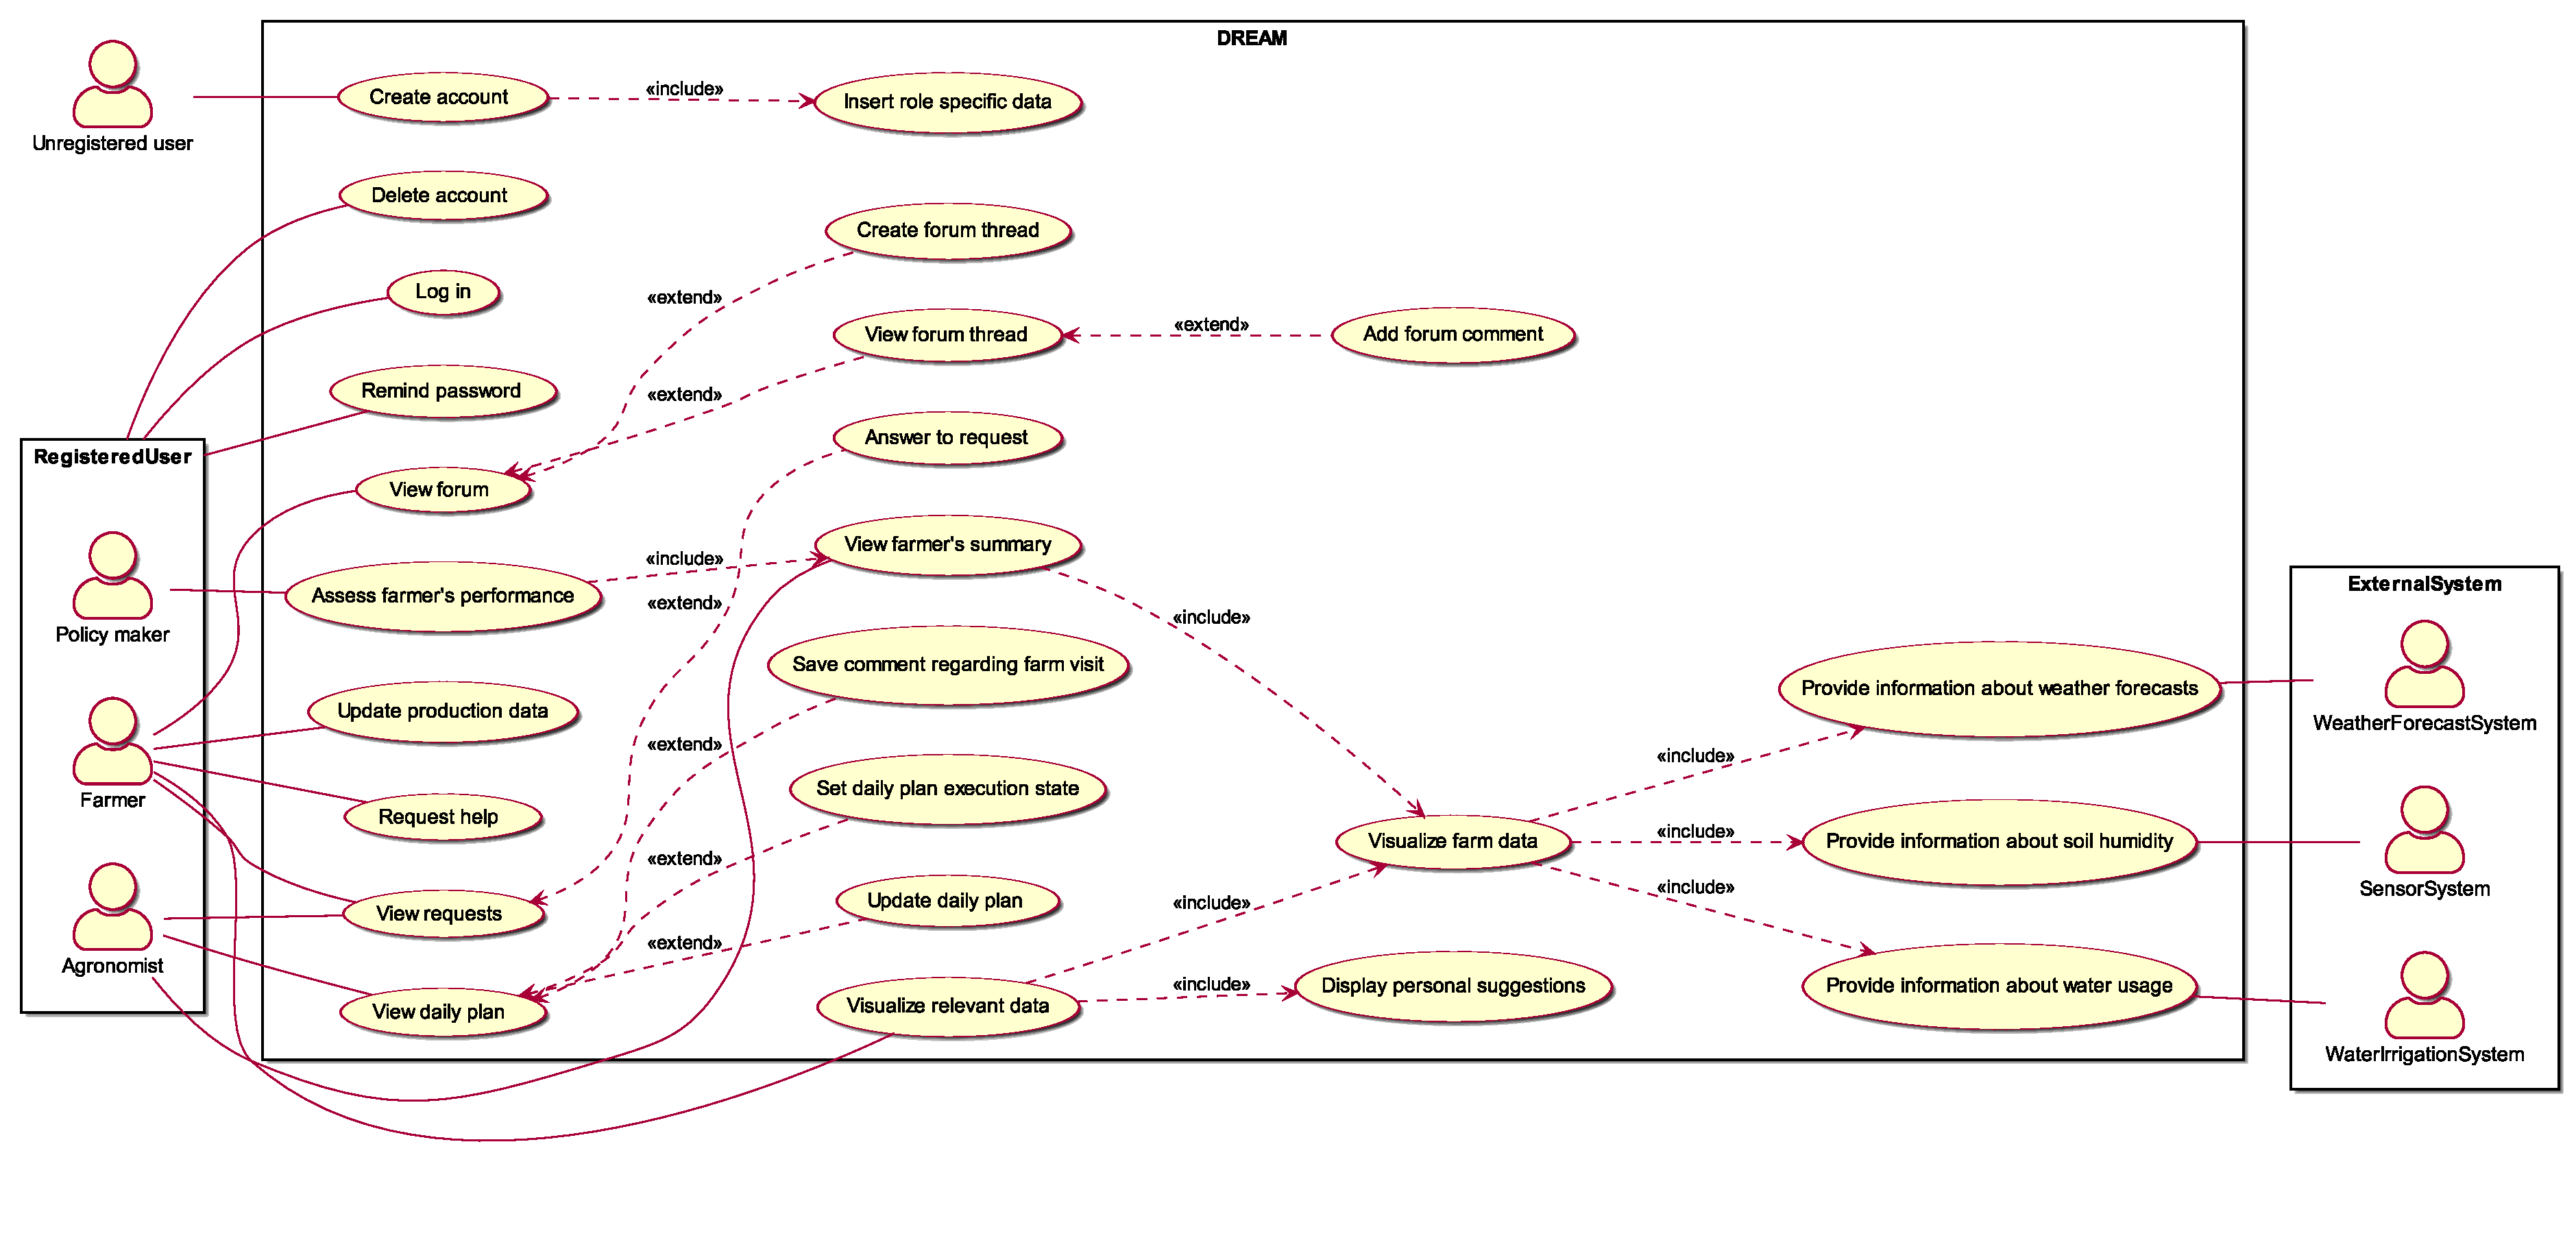
\includegraphics[width=0.92\textheight, keepaspectratio, origin=c, angle=90]{diagrams/use_case}
    \caption{Use case diagram}
    \label{fig:uc_diagram}
\end{figure}

% Definition of use case diagrams, 
% use cases and associated sequence/activity diagrams, 
% and mapping on requirements

\begin{figure}[H]
    \centering
    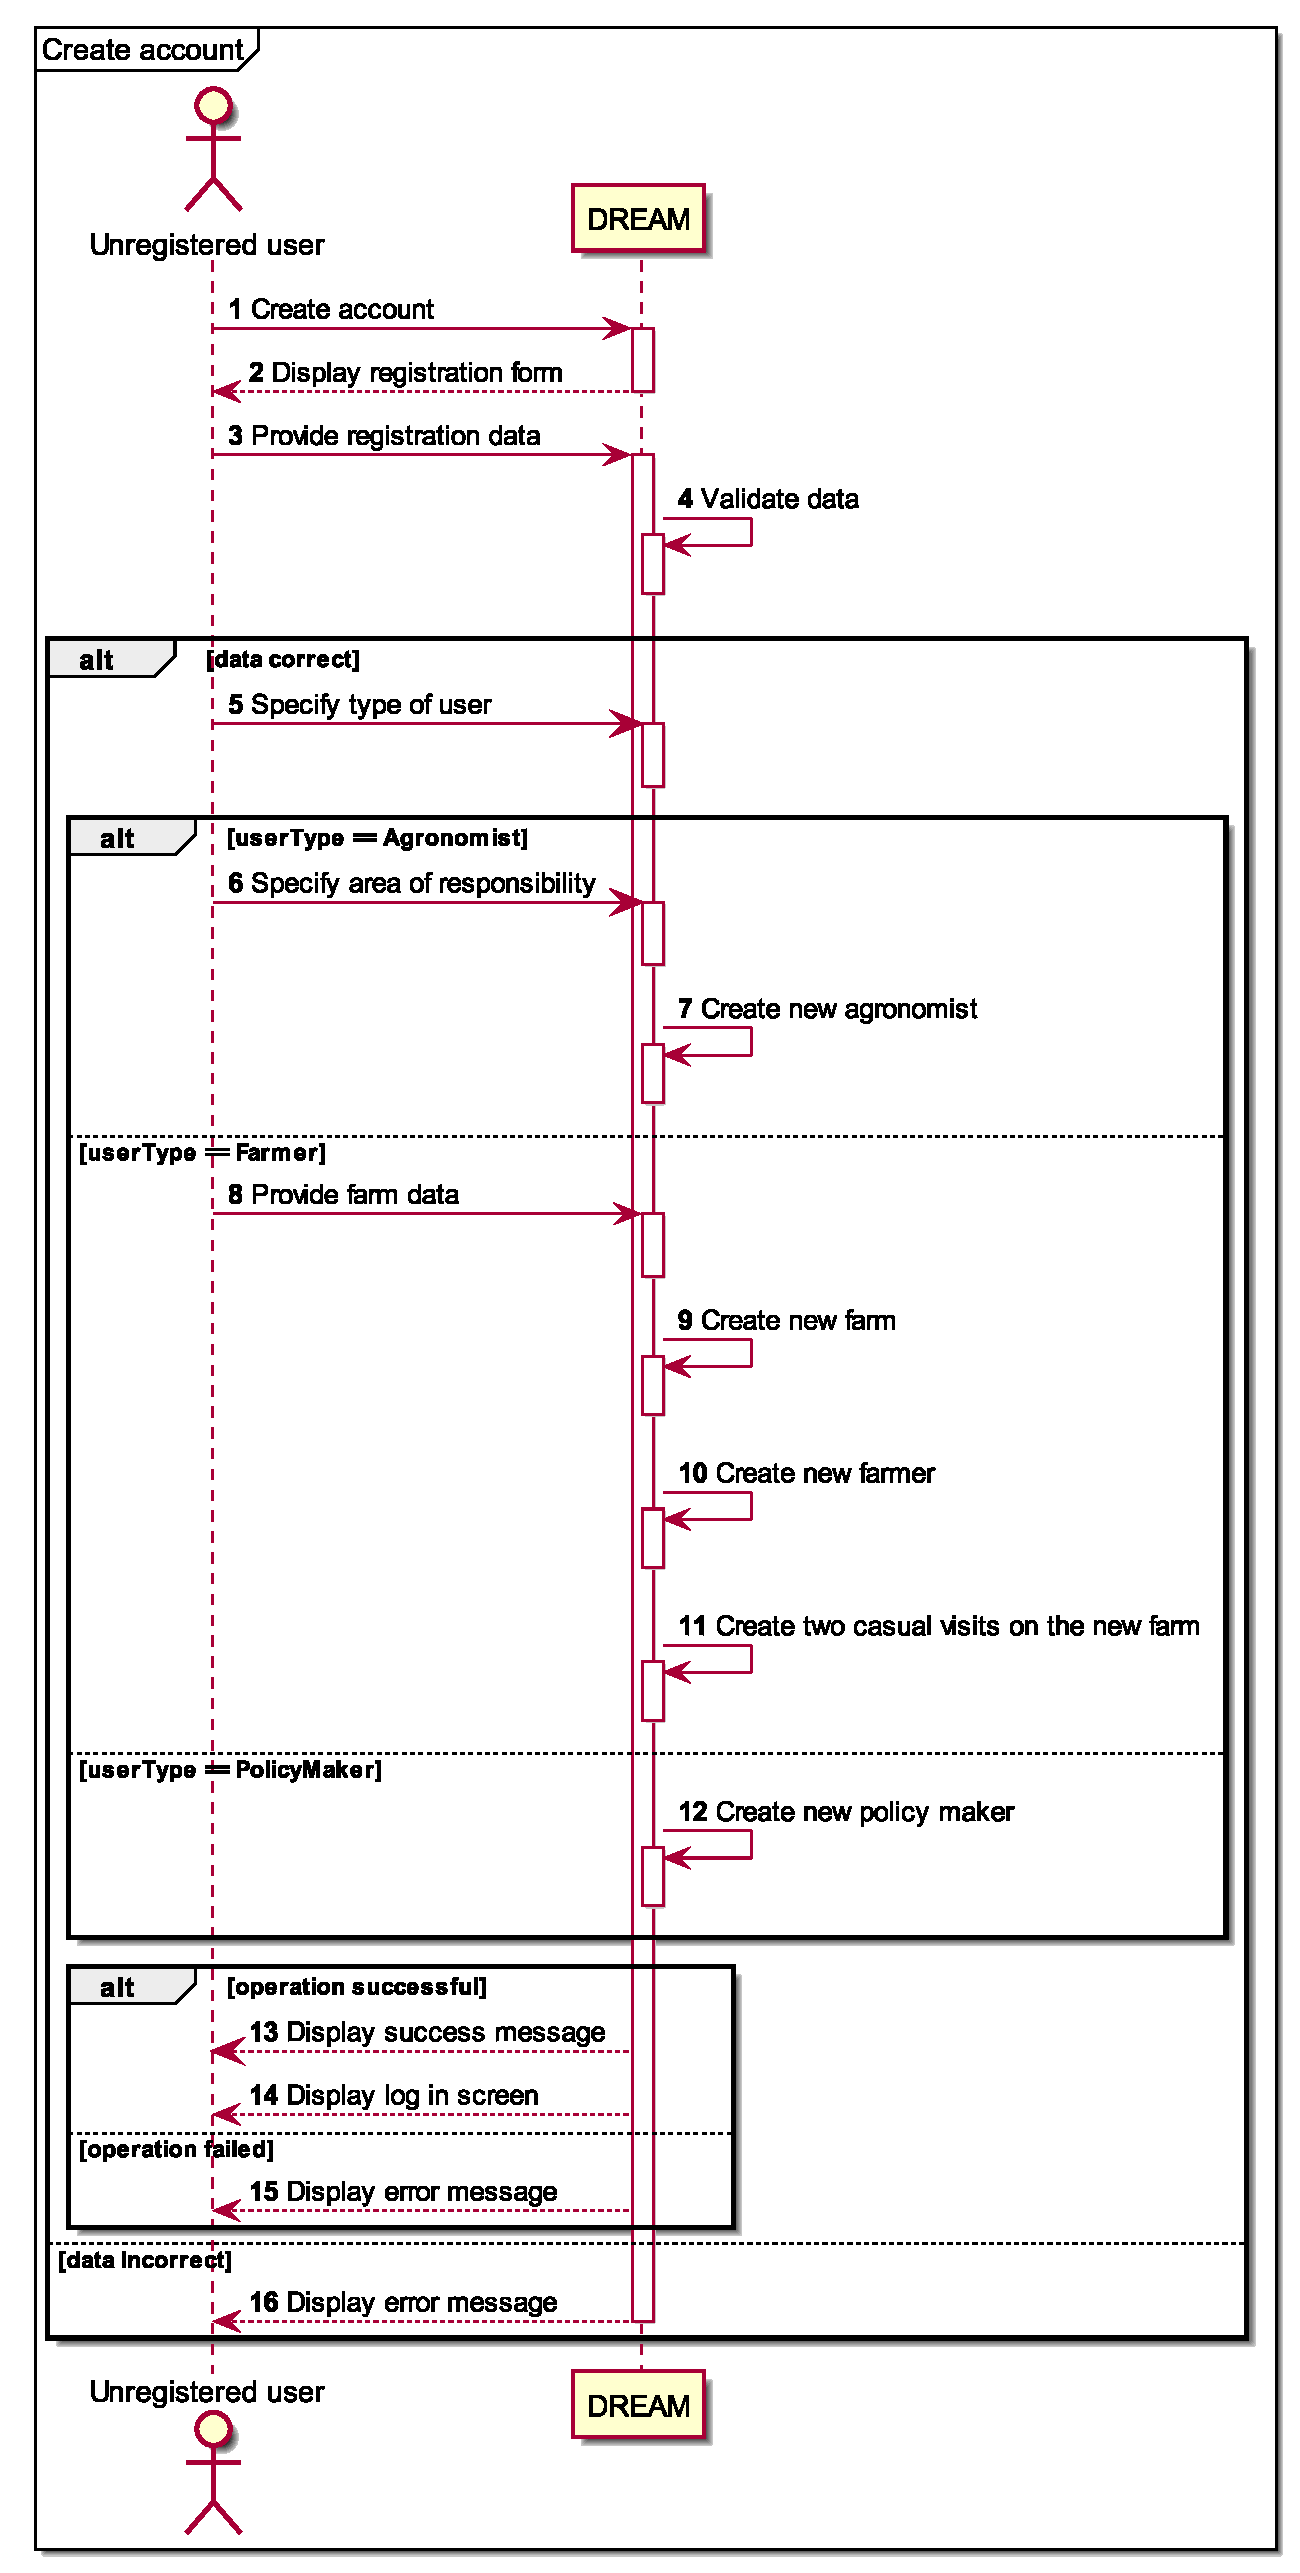
\includegraphics[scale=0.5, keepaspectratio, origin=c]{diagrams/sequence/create_account}
    \caption{Sequence diagram presenting the process of creating a new user account.}
    \label{fig:sd_create_account}
\end{figure}

\begin{figure}[H]
    \centering
    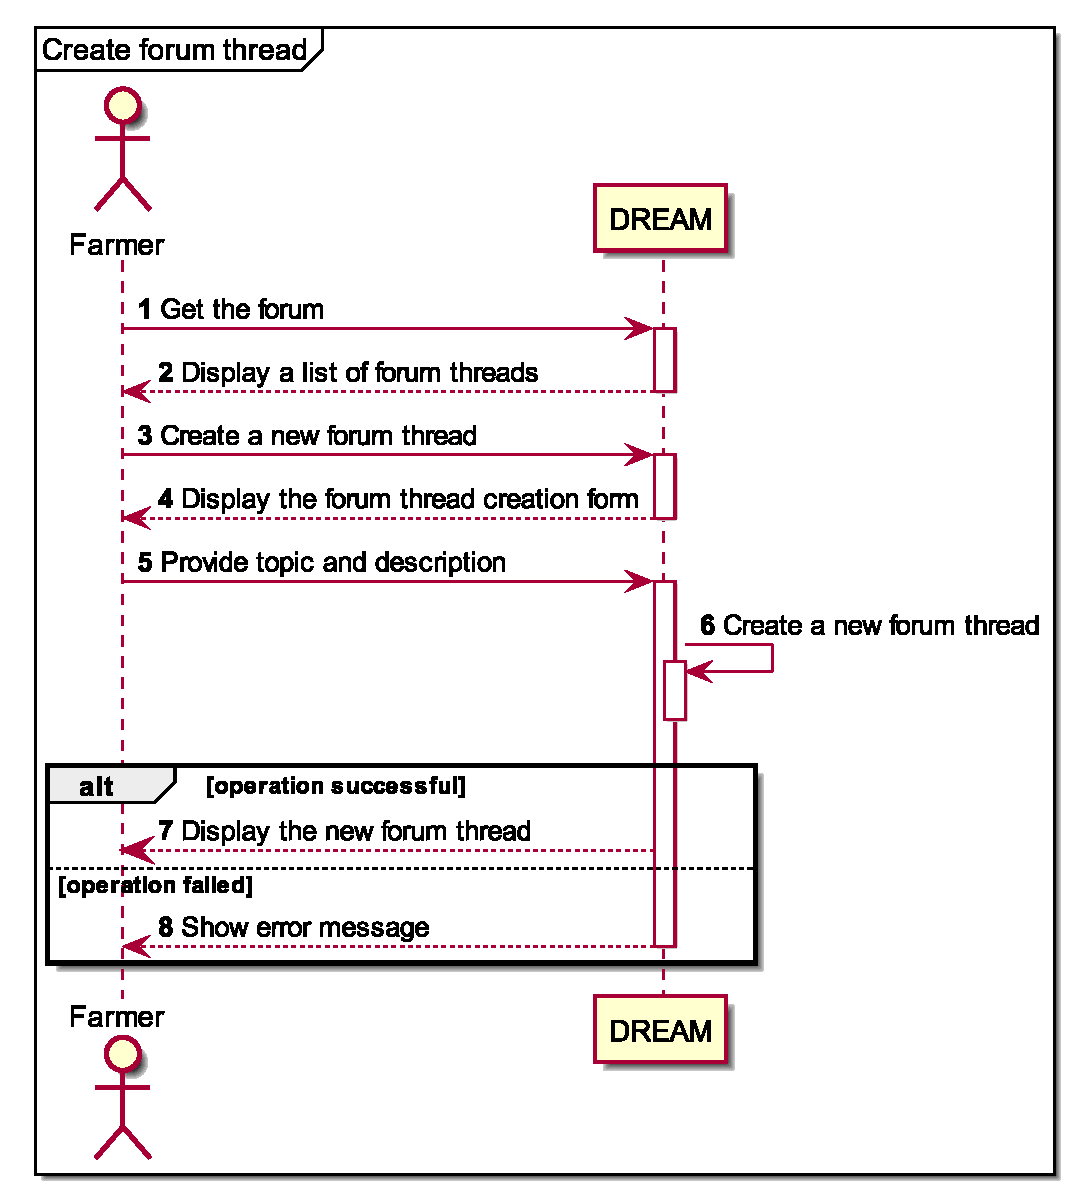
\includegraphics[scale=0.6, keepaspectratio, origin=c]{diagrams/sequence/create_forum_thread}
    \caption{Sequence diagram presenting the process of creating a new forum thread.}
    \label{fig:sd_create_forum_thread}
\end{figure}

\begin{figure}[H]
    \centering
    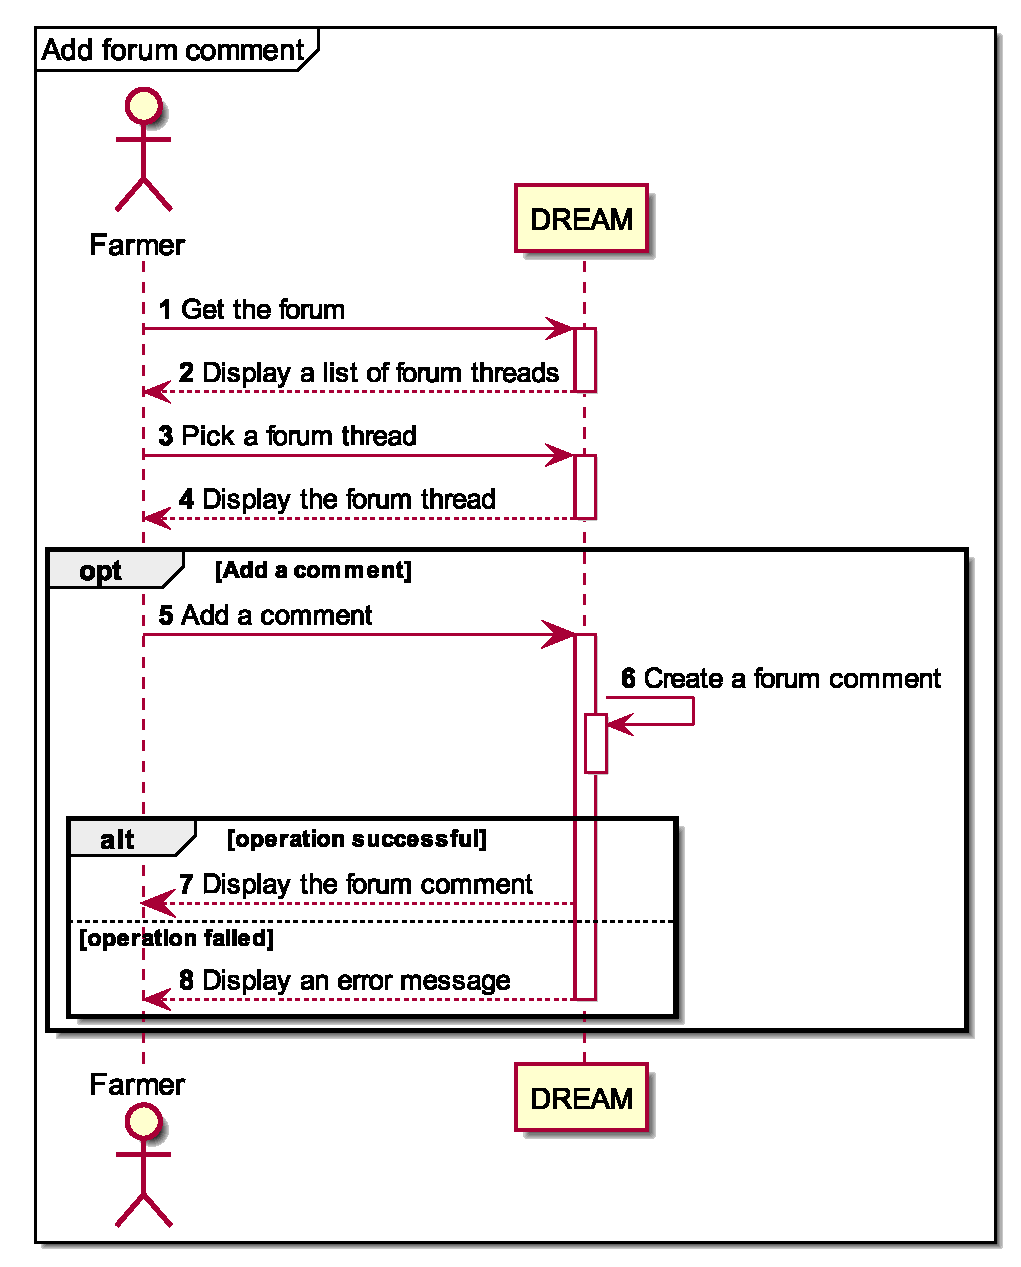
\includegraphics[scale=0.6, keepaspectratio, origin=c]{diagrams/sequence/add_forum_comment}
    \caption{Sequence diagram presenting the addition of a comment in a forum thread.}
    \label{fig:sd_add_forum_comment}
\end{figure}

\begin{figure}[H]
    \centering
    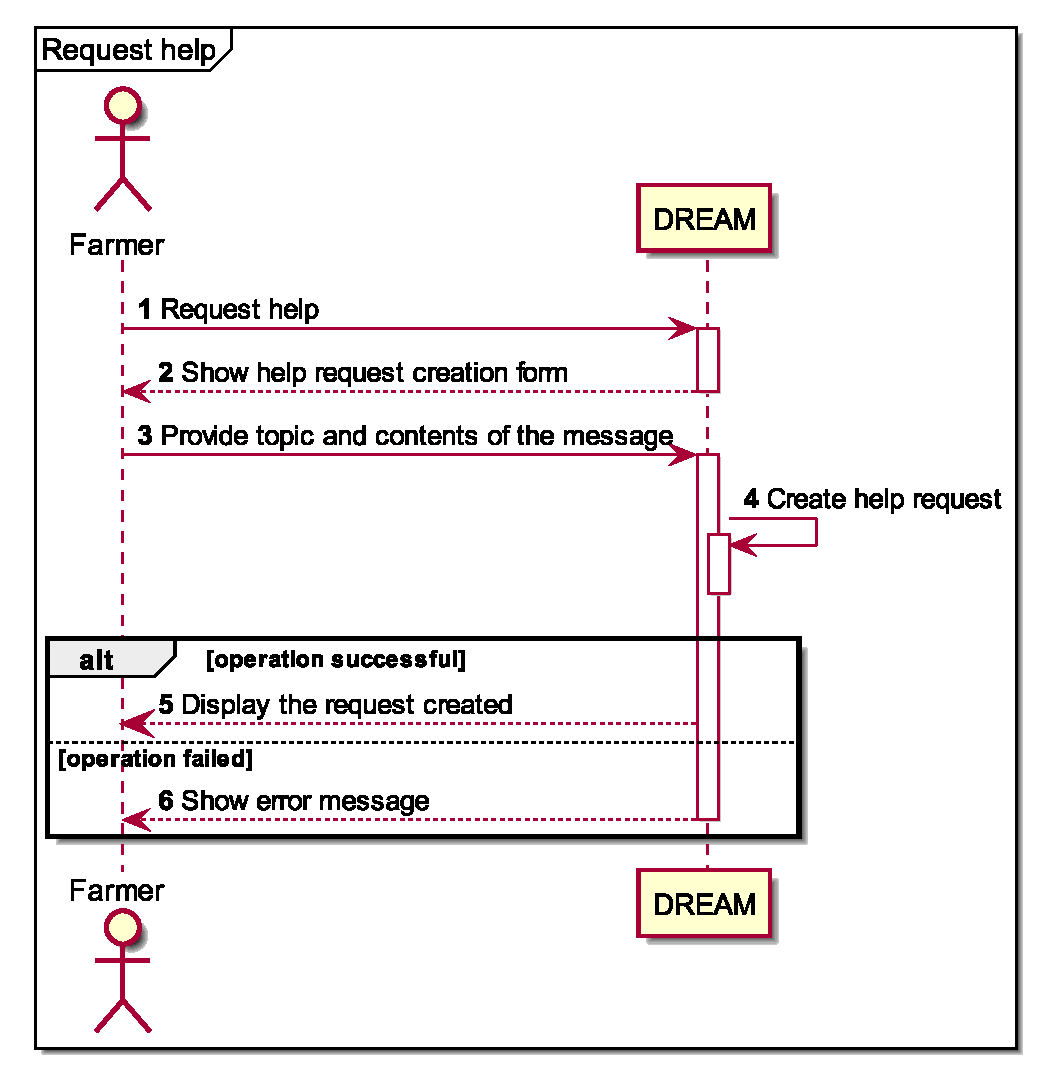
\includegraphics[scale=0.6, keepaspectratio, origin=c]{diagrams/sequence/request_help}
    \caption{Sequence diagram presenting the creation of a help request.}
    \label{fig:sd_request_help}
\end{figure}

\begin{figure}[H]
    \centering
    \includegraphics[scale=0.6, keepaspectratio, origin=c]{diagrams/sequence/answer_to_request}
    \caption{Sequence diagram presenting the event of answering to a help request.}
    \label{fig:sd_answer_to_request}
\end{figure}

\begin{figure}[H]
    \centering
    \includegraphics[scale=0.6, keepaspectratio, origin=c]{diagrams/sequence/view_daily_plan}
    \caption{Sequence diagram presenting the action of displaying a daily plan.}
    \label{fig:sd_view_daily_plan}
\end{figure}

\begin{figure}[H]
    \centering
    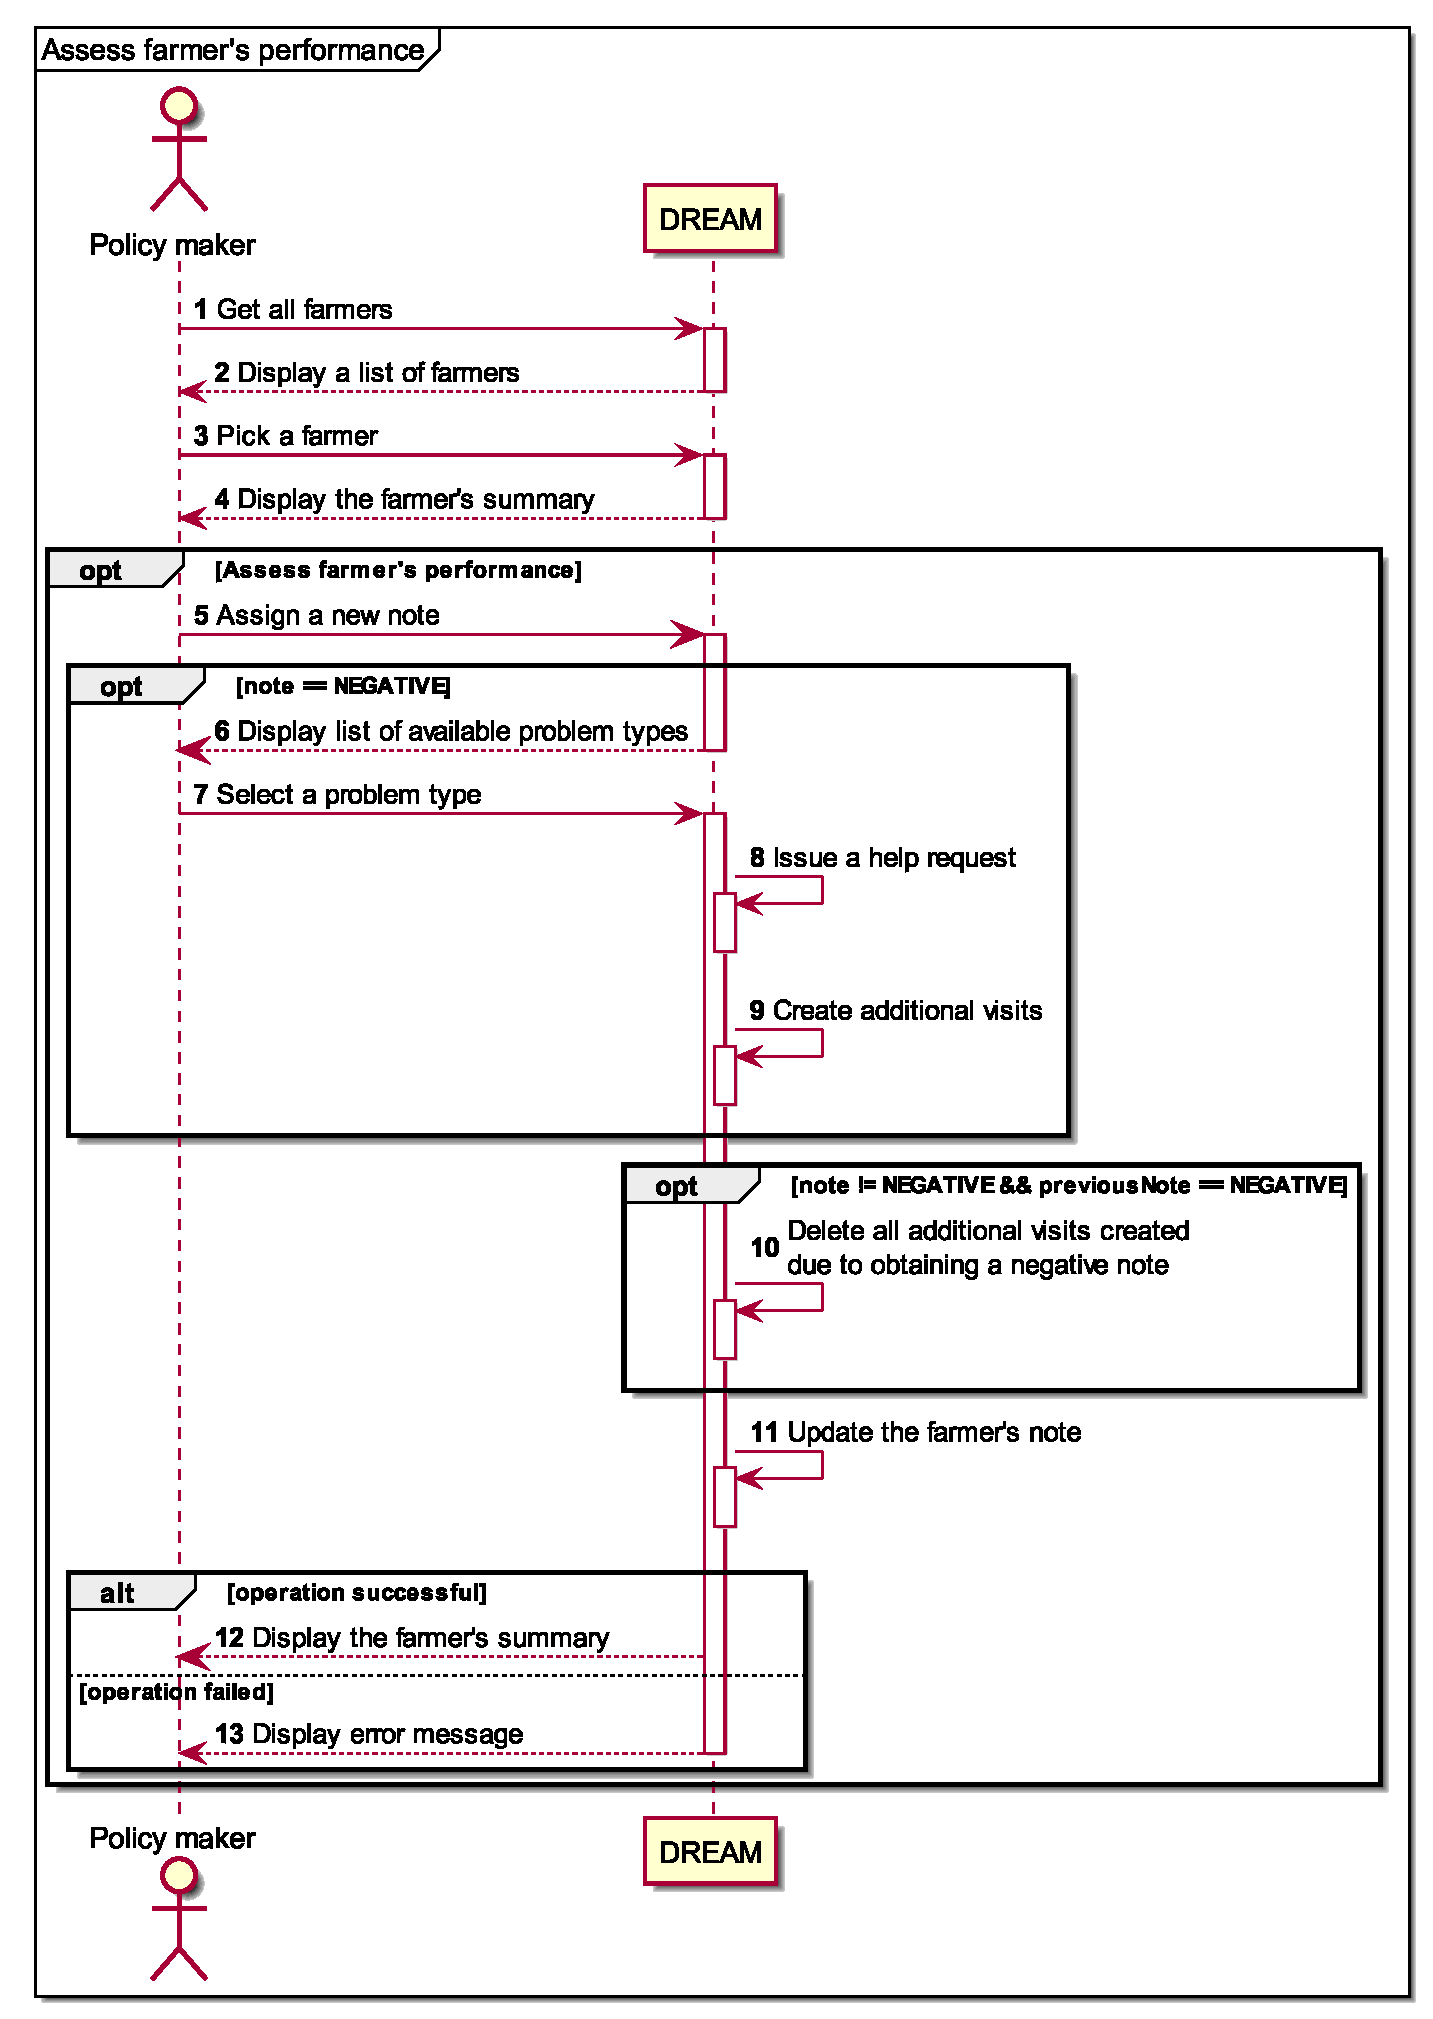
\includegraphics[scale=0.6, keepaspectratio, origin=c]{diagrams/sequence/assess_farmers_performance}
    \caption{Sequence diagram presenting farmer's performance assessment.}
    \label{fig:sd_assess_farmers_performance}
\end{figure}


\begin{table}[H]
    \centering
	\begin{tabular}{@{}p{0.25\linewidth} p{0.72\linewidth}@{}}
		\toprule
		\textbf{Name}               & Create account \\
		\midrule
		\textbf{Actors}             & Unregistered user \\
		\midrule
		\textbf{Goals}              & TODO \\
		\midrule
		
		\textbf{Entry conditions}   & \begin{itemize}[leftmargin=.4cm,noitemsep,topsep=0pt,before=\vspace{-3mm},after=\vspace{-4mm}]
		    \item The unregistered user, who wants to create an account, is  on the welcome screen of the application. \todo{check if it is consistent with UI mocks}
		\end{itemize}\\
		\midrule
		
		\textbf{Flow of events}     & \begin{enumerate}[leftmargin=.4cm,noitemsep,topsep=0pt,before=\vspace{-3mm},after=\vspace{-4mm}]
		    \item The unregistered user clicks on \textit{Sign up} button.
		    \item The application shows a form with role-irrelevant data (email, name, surname and password) to fill and a dropdown to choose the role.
		    \item The unregistered user fills the form and selects a role.
		    \item If a role of a farmer was chosen, the application shows another screen with text fields related to farm data to be filled.
		    \item If a role of an agronomist was chosen, the application shows another screen that asks to add the mandals to the agronomist's area of responsibility.
		    \item The unregistered user fills role-related data if there is any.
		    \item If a role of a farmer was chosen, the system creates a farm for a farmer.
		    \item If a role of an agronomist was chosen, the system adds selected mandals to the agronomist's area of responsibility.
		    \item The unregistered user clicks on \textit{Register} button.
		    \item The application creates a new user.
		    \item The application shows a message indicating successful registration.
		    \item The application shows the log in screen.
		\end{enumerate}\\
		\midrule
		\textbf{Exit conditions}    & A new user is created in the system. From now on, the credentials entered during the registration process can be used to log in to the application. \\
		\midrule
		
		\textbf{Exceptions}         & \begin{itemize}[leftmargin=.4cm,noitemsep,topsep=0pt,before=\vspace{-3mm}]
		   \item The unregistered user resigns from registration in the application by clicking the left arrow next to the view title. 
		\end{itemize}
		The application shows the log in screen.\begin{itemize}[leftmargin=.4cm,noitemsep,topsep=0pt]
		   \item The user with the given email adress already exists. 
		\end{itemize}
		The application shows a message explaining that the user with given email already exists.
	    \begin{itemize}[leftmargin=.4cm,noitemsep,topsep=0pt]
		   \item The application is not able to create a new user in step 10. 
		\end{itemize}
		The application shows a message indicating a possible cause of error.
	    \\\bottomrule
	\end{tabular}
	\caption{Use case description: create account} 
\end{table}


\begin{table}[H]
    \centering
	\begin{tabular}{@{}p{0.25\linewidth} p{0.72\linewidth}@{}}
\toprule
		\textbf{Name}               & Assess farmer's performance \todo{check if it's consistent with UI mocks}\\
		\midrule
		\textbf{Actors}             & Policy maker\\
		\midrule
		\textbf{Goals}              & TODO \\
		\midrule
		
		\textbf{Entry conditions}   & \begin{itemize}[leftmargin=.4cm,noitemsep,topsep=0pt,before=\vspace{-3mm},after=\vspace{-4mm}]
		    \item The policy maker is already logged in to the application.
		    \item The policy maker is in the list of farmers' view. 
		\end{itemize}\\
		\midrule
		
		\textbf{Flow of events}     & \begin{enumerate}[leftmargin=.4cm,noitemsep,topsep=0pt,before=\vspace{-3mm},after=\vspace{-4mm}]
		    \item The policy maker clicks on one of the farmers.
		    \item The application shows the selected farmer's summary.
		    \item The policy maker chooses a note from a dropdown.
		    \item The policy maker clicks on \textit{Save} button.
		    \item The application saves a new farmer's note.
		    \item The application shows a message indicating successful assignment of the note.
		\end{enumerate}\\
		\midrule
		\textbf{Exit conditions}    & The new note is saved in the system. In case of negative note assignment, it sends a help request to agronomists in the given area of responsibility and several well-performing farmers. \\
		\midrule
		
		\textbf{Exceptions}         & \begin{itemize}[leftmargin=.4cm,noitemsep,topsep=0pt,before=\vspace{-3mm}]
		   \item The policy maker resigns from changing the current note held by a farmer by clicking the left arrow next to the view title. 
		\end{itemize}
	    The system comes back to the list of farmers' view.
	    \begin{itemize}[leftmargin=.4cm,noitemsep,topsep=0pt]
		   \item The application is not able to save note assigned in step 5. 
		\end{itemize}
		The application shows a message indicating a possible cause of error.
		\\\bottomrule
	\end{tabular}
	\caption{Use case description: assess farmer's performance} 
\end{table}

\begin{table}[H]
    \centering
	\begin{tabular}{@{}p{0.25\linewidth} p{0.72\linewidth}@{}}
\toprule
		\textbf{Name}               & Create forum thread\\
		\midrule
		\textbf{Actors}             & Farmer\\
		\midrule
		\textbf{Goals}              & TODO \\
		\midrule
		
		\textbf{Entry conditions}   & \begin{itemize}[leftmargin=.4cm,noitemsep,topsep=0pt,before=\vspace{-3mm},after=\vspace{-4mm}]
		    \item The farmer is already logged in to the application.
		    \item The farmer is in the \textit{Forum} view, accessible from the sidebar of the application.
		\end{itemize}\\
		\midrule
		
		\textbf{Flow of events}     & \begin{enumerate}[leftmargin=.4cm,noitemsep,topsep=0pt,before=\vspace{-3mm},after=\vspace{-4mm}]
		    \item The farmer clicks on \textit{Create forum thread} at the bottom of the page.
		    \item The application shows a pop-up with textboxes to fill.
		    \item The farmer enters the topic and description of the thread.
		    \item The farmer clicks on \textit{Create} button.
		    \item The application creates a new forum thread.
		    \item The application shows a message indicating successful creation of the forum thread.
		\end{enumerate}\\
		\midrule
		\textbf{Exit conditions}    & The application successfully created a new forum thread. From now on, the new forum thread is visible to all other farmers. \\
		\midrule
		
		\textbf{Exceptions}         & \begin{itemize}[leftmargin=.4cm,noitemsep,topsep=0pt,before=\vspace{-3mm}]
		   \item The farmer closes the pop-up showed in step 2.
		\end{itemize}
	    The system comes back to the \textit{Forum} view.
	    \begin{itemize}[leftmargin=.4cm,noitemsep,topsep=0pt]
		   \item The application is not able to create a forum thread in step 5. 
		\end{itemize}
		The application shows a message indicating a possible cause of error.
        \\\bottomrule
	\end{tabular}
	\caption{Use case description: create forum thread} 
\end{table}


\begin{table}[H]
    \centering
	\begin{tabular}{@{}p{0.25\linewidth} p{0.72\linewidth}@{}}
\toprule
		\textbf{Name}               & Add forum comment \\
		\midrule
		\textbf{Actors}             & Farmer\\
		\midrule
		\textbf{Goals}              & TODO \\
		\midrule
		
		\textbf{Entry conditions}   & \begin{itemize}[leftmargin=.4cm,noitemsep,topsep=0pt,before=\vspace{-3mm},after=\vspace{-4mm}]
		    \item The farmer is already logged in to the application.
		    \item The farmer is in the \textit{Forum} view, accessible from the sidebar of the application.
		\end{itemize}\\
		\midrule
		
		\textbf{Flow of events}     & \begin{enumerate}[leftmargin=.4cm,noitemsep,topsep=0pt,before=\vspace{-3mm},after=\vspace{-4mm}]
		    \item The farmer selects a forum thread, by clicking on the tread's topic in the list.
		    \item The application shows the contents of the selected forum thread.
		    \item The farmer fills the textbox with the content of his comment.
		    \item The farmer clicks on \textit{Send} button.
		    \item The application adds a new forum comment.
		    \item The application shows a message indicating successful addition of the forum comment.
		\end{enumerate}\\
		\midrule
		\textbf{Exit conditions} & The application saved the new comment in the thread. From now on, the new comment is visible to all farmers viewing the thread. \\
		\midrule
		
		\textbf{Exceptions}         & \begin{itemize}[leftmargin=.4cm,noitemsep,topsep=0pt,before=\vspace{-3mm}]
		   \item The farmer cancels the operation, clicking on a left arrow next to the thread's title.
		\end{itemize}
	    The system comes back to the \textit{Forum} view.
	    \begin{itemize}[leftmargin=.4cm,noitemsep,topsep=0pt]
		   \item The application is not able to add a forum comment in step 5. 
		\end{itemize}
		The application shows a message indicating a possible cause of error.
		\\\bottomrule
	\end{tabular}
	\caption{Use case description: add forum comment} 
\end{table}

\begin{table}[H]
    \centering
	\begin{tabular}{@{}p{0.25\linewidth} p{0.72\linewidth}@{}}
\toprule
		\textbf{Name}               & Request help\\
		\midrule
		\textbf{Actors}             & Farmer\\
		\midrule
		\textbf{Goals}              & TODO \\
		\midrule
		
		\textbf{Entry conditions}   & \begin{itemize}[leftmargin=.4cm,noitemsep,topsep=0pt,before=\vspace{-3mm},after=\vspace{-4mm}]
		    \item The farmer is already logged in to the application.
		\end{itemize}\\
		\midrule
		
		\textbf{Flow of events}     & \begin{enumerate}[leftmargin=.4cm,noitemsep,topsep=0pt,before=\vspace{-3mm},after=\vspace{-4mm}]
		    \item The farmer clicks on \textit{My help requests} view in the sidebar.
		    \item The farmer clicks on \textit{Create help request} button.
		    \item The application shows a pop-up with textboxes to fill.
		    \item The farmer enters topic and description of the problem.
		    \item The farmer clicks on \textit{Send request} button.
		    \item The application sends requests to the agronomists in the given area of responsibility and farmers with positive note. 
		    \item The application shows a message indicating successful sending of the message.
		\end{enumerate}\\
		\midrule
		\textbf{Exit conditions}    & The request can be seen in the \textit{Provide help} view by the recipients selected in step 6. Additionaly, the farmer who created the request can see it in the \textit{My help requests} view. \\
		\midrule
		
		\textbf{Exceptions}         & \begin{itemize}[leftmargin=.4cm,noitemsep,topsep=0pt,before=\vspace{-3mm}]
		   \item The farmer closes the pop-up showed in step 3.
		\end{itemize}
	    The system comes back to the \textit{My help requests} view.
	    \begin{itemize}[leftmargin=.4cm,noitemsep,topsep=0pt]
		   \item The application is not able to create a request for help in step 6. 
		\end{itemize}
		The application shows a message indicating a possible cause of error.\\
		\bottomrule
	\end{tabular}
	\caption{Use case description: request help} 
\end{table}

\begin{table}[H]
    \centering
	\begin{tabular}{@{}p{0.25\linewidth} p{0.72\linewidth}@{}}
\toprule
		\textbf{Name}               & Answer to request\\
		\midrule
		\textbf{Actors}             & Agronomist, Farmer\\
		\midrule
		\textbf{Goals}              & TODO \\
		\midrule
		
		\textbf{Entry conditions}   & \begin{itemize}[leftmargin=.4cm,noitemsep,topsep=0pt,before=\vspace{-3mm},after=\vspace{-4mm}]
		    \item The farmer or the agronomist is already logged in to the application.
		    \item The farmer or the agronomist is in the \textit{Provide help} view.
		\end{itemize}\\
		\midrule
		
		\textbf{Flow of events}     & \begin{enumerate}[leftmargin=.4cm,noitemsep,topsep=0pt,before=\vspace{-3mm},after=\vspace{-4mm}]
		    \item The farmer or the agronomist clicks on the requests he wants to reply. 
		    \item The application shows a pop-up with textboxes to fill.
		    \item The farmer or the agronomist enters the contents of the reply message.
		    \item The farmer or the agronomist clicks the \textit{Send} button.
		    \item The application sends an answer to the request to the farmer.
		    \item The application shows a message indicating successful sending of the message.
		\end{enumerate}\\
		\midrule
		\textbf{Exit conditions}    & The farmer can see the response by clicking on the request in the \textit{My help request tab}. \\
		\midrule
		
		\textbf{Exceptions}         & \begin{itemize}[leftmargin=.4cm,noitemsep,topsep=0pt,before=\vspace{-3mm}]
		   \item The farmer closes the pop-up showed in step 2.
		\end{itemize}
	    The system comes back to the \textit{Provide help} view.
	    \begin{itemize}[leftmargin=.4cm,noitemsep,topsep=0pt]
		   \item The application is not able to create an answer to a help request in step 5. 
		\end{itemize}
		The application shows a message indicating a possible cause of error.
		\\\bottomrule
	\end{tabular}
	\caption{Use case description: answer to request} 
\end{table}

\begin{table}[H]
    \centering
	\begin{tabular}{@{}p{0.25\linewidth} p{0.72\linewidth}@{}}
		\toprule
		\textbf{Name}               & Set daily plan execution state \\
		\midrule
		\textbf{Actors}             & Agronomist\\
		\midrule
		\textbf{Goals}              & TODO \\
		\midrule
		
		\textbf{Entry conditions}   & \begin{itemize}[leftmargin=.4cm,noitemsep,topsep=0pt,before=\vspace{-3mm},after=\vspace{-4mm}]
		    \item The farmer or the agronomist is already logged in to the application
		    \item TODO \todo{To be completed}
		\end{itemize}\\
		\midrule
		
		\textbf{Flow of events}     & \begin{enumerate}[leftmargin=.4cm,noitemsep,topsep=0pt,before=\vspace{-3mm},after=\vspace{-4mm}]
		    \item TODO
		\end{enumerate}\\
		\midrule
		\textbf{Exit conditions}    & TODO \\
		\midrule
		
		\textbf{Exceptions}         & \begin{itemize}[leftmargin=.4cm,noitemsep,topsep=0pt,before=\vspace{-3mm}]
		   \item TODO
		\end{itemize}
	    \\\bottomrule
	\end{tabular}
	\caption{Use case description: set daily plan execution state} 
\end{table}

\begin{table}[H]
    \centering
	\begin{tabular}{@{}p{0.25\linewidth} p{0.72\linewidth}@{}}
        \toprule
		\textbf{Name}               & Update daily plan\\
		\midrule
		\textbf{Actors}             & Agronomist\\
		\midrule
		\textbf{Goals}              & TODO \\
		\midrule
		
		\textbf{Entry conditions}   & \begin{itemize}[leftmargin=.4cm,noitemsep,topsep=0pt,before=\vspace{-3mm},after=\vspace{-4mm}]
		    \item The agronomist is already logged in to the application.
		    \item The agronomist is in the daily plan view.
		\end{itemize}\\
		\midrule
		
		\textbf{Flow of events}     & \begin{enumerate}[leftmargin=.4cm,noitemsep,topsep=0pt,before=\vspace{-3mm},after=\vspace{-4mm}]
		    \item The agronomist clicks on the day in the calendar in which he wants to rearrange the visits.
		    \item The application shows a pop-up with a list of visit in the selected day.
		    \item The agronomist selects a visit he wants to rearrange from the list.
		    \item The agronomist selects a new date for the visit selected in the previous step.
		    \item The agronomist confirms his choice.
		    \item The application saves changes made to the daily plan.
		    \item The application shows a message indicating successful save of the visit's date.
		\end{enumerate}\\
		\midrule
		\textbf{Exit conditions}    & The calendar in the \textit{Visit plan} view was modified accordingly. \\
		\midrule
		
		\textbf{Exceptions}         & \begin{itemize}[leftmargin=.4cm,noitemsep,topsep=0pt,before=\vspace{-3mm}]
		   \item An agronomist closes the popup shown in the step 2, 3 or 4.
		\end{itemize}
	    The system shows the daily plan tab view. \begin{itemize}[leftmargin=.4cm,noitemsep,topsep=0pt]
		   \item An agronomist wants to rearrange the visit to a farm, although it was not visited twice a year.
		\end{itemize}
		The application shows a warning.
	    \begin{itemize}[leftmargin=.4cm,noitemsep,topsep=0pt]
		   \item The application is not able to save updates to the daily plan in step 6. 
		\end{itemize}
		The application shows a message indicating a possible cause of error.
		\\\bottomrule
	\end{tabular}
	\caption{Use case description: update daily plan} 
\end{table}


\begin{table}[H]
    \centering
	\begin{tabular}{@{}p{0.25\linewidth} p{0.72\linewidth}@{}}
        \toprule
		\textbf{Name}               & Save comment regarding farm visit\\
		\midrule
		\textbf{Actors}             & Agronomist\\
		\midrule
		\textbf{Goals}              & TODO \\
		\midrule
		
		\textbf{Entry conditions}   & \begin{itemize}[leftmargin=.4cm,noitemsep,topsep=0pt,before=\vspace{-3mm},after=\vspace{-4mm}]
		    \item The agronomist is already logged in to the application.
		    \item The agronomist is in the daily plan view.
		\end{itemize}\\
		\midrule
		
		\textbf{Flow of events}     & \begin{enumerate}[leftmargin=.4cm,noitemsep,topsep=0pt,before=\vspace{-3mm},after=\vspace{-4mm}]
		    \item TODO 
		\end{enumerate}\\
		\midrule
		\textbf{Exit conditions}    & The information obtained during a visit to a farm is saved in the system. \\
		\midrule
		
		\textbf{Exceptions}         & \begin{itemize}[leftmargin=.4cm,noitemsep,topsep=0pt,before=\vspace{-3mm}]
		    \item An agronomist cancels the operation during the step TODO.
		\end{itemize}
	    The system shows the daily plan view.
	    \begin{itemize}[leftmargin=.4cm,noitemsep,topsep=0pt]
		   \item The application is not to save comment regarding a farm visit. 
		\end{itemize}
		The application shows a message indicating a possible cause of error.
		\\ \bottomrule
	\end{tabular}
	\caption{Use case description: save comment regarding farm visit} 
\end{table}

\subsection{Mapping on requirements}
% \begin{center}
% 	\begin{tabular}{@{}p{0.06\linewidth} p{0.44\linewidth} p{0.44\linewidth}@{}}
% 		\toprule
% 		\textbf{Goal}   & \textbf{Domain assumption} & \textbf{Requirement} \\
% 		\midrule
% 		\autonum{G} & A1, A2, A3, A4, A5, A6, A7, A10, A11, A14 & \\
% 		\autonum{G} & A1, A2, A3, A4, A6, A7, A8  & \\
% 		\autonum{G} & A1, A2, A3, A4, A5, A7, A9, A12, A13, A16  & \\
% 		\autonum{G} & A12, A15, A16  & \\
% 		\bottomrule
% 	\end{tabular}
% \end{center}

\begin{table}[H]
    \centering
    \begin{tabularx}{\linewidth}{lX} \toprule
         \textbf{G1} & Acquire, combine, and visualize data both from external systems and users. \\ \midrule
         \textbf{A1} & Each farmer possess exactly one farm. \\
         \textbf{A2} & Each farm belongs to exactly one farmer. \\
         \textbf{A3} & Each farm has at least one humidity sensor. \\
         \textbf{A4} & Each farm has an irrigation system. \\
         \textbf{A5} & Each farm is inside exactly one mandal. \\
         \textbf{A6} & Each farmer updates his production data each month. \\
         \textbf{A7} & Weather is consistent in a given mandal.\\
         \textbf{A10} & Each registered user can be only one of the actors: an agronomist, a farmer, or a policy maker. \\
         \textbf{A11} & The information provided by a user during registration process is valid. \\
         \textbf{A14} & Based on farmer's summary, a policy maker is able to understand whether the help given by farmers and agronomists produces significant results.\\ 
         \midrule
         \textbf{R1} & Each user is uniquely identified by his e-mail in the system. \\
         \textbf{R2} & Unregistered customer is able to create an account with a chosen role in the system. \\
         \textbf{R4} &  The application requires a farmer to insert data regarding his farm during the registration process. \\
         \textbf{R5} & Registered user is able to log in to the application. \\
		 \textbf{R6} & Registered user is able to reset his password. \\
         \textbf{R9} & A farmer is able to see farmer's relevant data. \\
         \textbf{R10} & A farmer is able to update production data in a given month. \\
          \textbf{R24} & The application has a predefined list of suggestions for the farmers. \\
          \textbf{R31} & The application reads and updates  weather forecasts every day. \\
          \textbf{R32} & The application reads and stores  data from humidity sensors every day.  \\
          \textbf{R33} & The application stores data from irrigation systems every day. \\
         \bottomrule
    \end{tabularx}
    \caption{G1 mapping on assumptions and requirements.}
\end{table}

\begin{table}[H]
    \centering
    \begin{tabularx}{\linewidth}{lX} \toprule
         \textbf{G2} & Facilitate performance assessment of the farmers. \\ \midrule
         \textbf{A1} & Each farmer possess exactly one farm. \\ 
         \textbf{A2} & Each farm belongs to exactly one farmer. \\
         \textbf{A3} & Each farm has at least one humidity sensor.\\
         \textbf{A4} & Each farm has an irrigation system.\\
         \textbf{A5} & Each farm is inside exactly one mandal. \\
         \textbf{A6} & Each farmer updates his production data each month. \\
         \textbf{A7} & Weather is consistent in a given mandal.\\
         \textbf{A8} & Initially, each farmer has a neutral note.\\
         \textbf{A14} & Based on farmer's summary, a policy maker is able to understand whether the help given by farmers and agronomists produces significant results.\\ 
         \midrule
         \textbf{R7} & A policy maker is able to assign a note to a farmer. \\
		\textbf{R8} & A policy maker is able to see farmer's summary. \\
		\textbf{R10} & A farmer is able to update production data in a given month.\\
		\bottomrule
    \end{tabularx}
    \caption{G2 mapping on assumptions and requirements.}
\end{table}

\begin{table}[H]
\centering
    \begin{tabularx}{\linewidth}{lX} \toprule
         \textbf{G3} & Ensure regular support of farmers by agronomists. \\ \midrule
         \textbf{A1} & Each farmer possess exactly one farm. \\
         \textbf{A2} & Each farm belongs to exactly one farmer. \\
         \textbf{A3} & Each farm has at least one humidity sensor. \\
         \textbf{A4} & Each farm has an irrigation system. \\
         \textbf{A5} & Each farm is inside exactly one mandal. \\
         \textbf{A7} & Weather is consistent in a given mandal.\\
         \textbf{A9} & Agronomist's area of responsibility contains at least one mandal.\\
         \textbf{A12} & Well-performing farmers and agronomists are eager to help farmers with negative notes. \\
         \textbf{A13} & Each mandal has at least one agronomist who is responsible for the farms inside that area.\\
         \textbf{A16} & Farmers and agronomists create meaningful and not offensive help requests and responses.\\
         \midrule
         \textbf{R3} & The application requires from an agronomist  to choose the area of responsibility during the registration process. \\
         \textbf{R10} & A farmer is able to update production data in a given month.\\
          \textbf{R11} &  A farmer is able to create a request for help. \\
         \textbf{R} & An agronomist is able to respond to a request for help. \\
         \textbf{R17} & An agronomist is able to see previous requests for help. \\
         \textbf{R18} & An agronomist is able to see his daily plan. \\
         \textbf{R19} & An agronomist is able to save comments regarding a farm visit. \\
         \textbf{R20} & An agronomist is able to set his daily plan's execution state. \\
         \textbf{R21} & An agronomist is able to update the daily plan. \\
         \textbf{R22} & An agronomist is able to see farmer's summary. \\
          \textbf{R25} & The application creates requests for help for farmers that obtained a negative note. \\
          \textbf{R26} &  The application selects recipients of requests for help based on agronomists' areas of responsibility and farmers' notes. \\
          \textbf{R27} &  The application schedules farm visits after each creation of a new farm. \\
          \textbf{R28} &  Aplication schedules new farm visits after each confirmation of a farm visit. \\
          \textbf{R29} &  The application schedules new farm visits after each confirmation and rejection of a farm visit. \\
          \textbf{R30} &  The application shows a warning if an agronomist wants to rearrange the visit to a farm, although it was not visited twice a year. \\
         \bottomrule
    \end{tabularx}
    \caption{G3 mapping on assumptions and requirements}
\end{table}

\begin{table}[H]
    \centering
    \begin{tabularx}{\linewidth}{lX} \toprule
         \textbf{G4} & Enable farmers to exchange their knowledge. \\ \midrule
         \textbf{A12} &  Well-performing farmers and agronomists are eager to help farmers with negative notes.\\ 
         \textbf{A15} & Farmers create meaningful and not offensive threads and comments on the forum.\\
         \textbf{A16} & Farmers and agronomists create meaningful and not offensive help requests and responses. \\
         \midrule
          \textbf{R11} &  A farmer is able to create a request for help. \\
          \textbf{R12} & A farmer is able to see previous requests for help. \\
          \textbf{R13} & A farmer with a positive note is able to respond to a request for help. \\
          \textbf{R14} & A farmer is able to create a forum thread. \\
		 \textbf{R15} & A farmer is able to see forum threads and their contents. \\
		 \textbf{R16} & A farmer is able to create a comment in a forum thread. \\ 
          \textbf{R25} & The application creates requests for help for farmers that obtained a negative note. \\
          \textbf{R26} &  The application selects recipients of requests for help based on agronomists' areas of responsibility and farmers' notes. \\
         \bottomrule
    \end{tabularx}
    \caption{G4 mapping on assumptions and requirements}
\end{table}

\section{Performance Requirements} \label{sec:performance_requirements}

Given that the system is intended for Telangana farmers, agronomists, and policymakers, it is fair to assume that it will be utilized by about 30 000 people. Therefore, the following performance requirements, which were formulated taking into consideration the best practices \cite{performance_requirements}, should be met.

\subsection{Response Time}

\begin{itemize}
    \item During peak hours, the average response time should be 2 seconds.
    \item During peak hours, 99\% of all response times must be shorter than 3 seconds.
    \item In each 10-minute period commencing on the hour, the average response time must be 2 seconds or less.
    \item 95\% percent of all response times must be shorter than 2 seconds.
\end{itemize}
 
\subsection{Workload}

\begin{itemize}
    \item The system must be capable of processing 20 transactions per second.
    \item The system must have no more than one hour of downtime every three months.
\end{itemize}

\subsection{Scalability}

\begin{itemize}
    \item The system must be able to sustain a 5\% yearly growth in new users.
    \item The system must be able to sustain a 10\% yearly increase in the number of transactions per second.
    \item The system shall be able to extend its connections to new external systems providing relevant data as their number may arise.
\end{itemize}

\subsection{Platform}

DREAM has to be housed on a platform that meets the following criteria:

\begin{itemize}
    \item Operating system: Windows 10 or Windows 11.    
    \item \textit{.NET 6.0} development platform installed.
    \item \textit{PostgreSQL} object-relational database system.
    \item CPU: 1.4 GHz 64-bit processor compatible with x64 instruction set.
    \item Memory: Minimum 8 GB of RAM. 
    \item Hard drive space: minimum of 20 GB of space.
    \item Network adapter: an Ethernet adapter capable of at least 1 gigabit per second throughput.
\end{itemize}

\section{Design Constraints}

This section describes the constraints of a design. These include uncontrolled limitations that are self-imposed in order to enhance the design.

\subsection{Standards compliance}

The system will collect data from external systems and sensors, as well as data entered by users during registration and application use, such as production data, agronomist's daily plan, farmer's summary, and notes. The data will be used exclusively for system purposes and will be treated discreetly in accordance with the General Data Protection Regulation \cite{GDPR} and IS 17428.1 \cite{india_privacy_doc} guidelines. In particular, no information relating to a specific person will be made public as a result of the statistical analyses undertaken.

\subsection{Hardware limitations}

The following are the hardware constraints that the end user must meet in order to use the system.

\begin{itemize}
    \item Processor: 1.9 GHz x86- or x64-bit dual-core processor.
    \item Memory: 2 GB of RAM.
    \item Network: wired or wireless connection with bandwidth greater than 40 KBps (320 kbps) and latency under 200 ms.
    \item Web browser: Google Chrome, Firefox, Safari, Microsoft Edge, or Opera running on Windows, macOS, Linux, or mobile operating systems including Android and iOS, with \textit{JavaScript} enabled.
\end{itemize}

\subsection{Any other constraints}

DREAM will employ stateless protocols to enable components to be handled and changed without impacting the overall system. Additionally, the system will catalog, retrieve and run queries on all the relevant data using a relational database.

\section{Software System Attributes}

The system's characteristics that facilitate the measurement of its performance are presented in this section.

\subsection{Reliability}

The mean time between failures shall be equal to 120 hours, which means that in the worst case scenario it may break once every 5 days. Furthermore, the system shall be fault-tolerant, with its architecture prepared for any potential damage to system components by having replicas ready to be substituted. In order to recover from eventual data losses, redundancy should be considered for the system's database implementation.

\subsection{Availability}

As mentioned in the section \ref{sec:performance_requirements}, the system shall have no more than one hour of downtime every three months, thus, shall be highly available. In case of any planned maintenance works, all the users should be notified at least 48 hours in advance.

\subsection{Security}

The system shall implement role-based access control, which is a method of restricting system access to authorized users and granting permissions based on the user's role. It is accomplished through the use of both authentication and authorization implemented in the backend. The former is based on verifying the identity of a user, which can be an agronomist, a farmer, or a policy maker, during the log in phase. The latter, on the other hand, validates the logged-in user's permissions to perform an action (for example, visualizing an agronomist's daily plan) before actually carrying it out.

\subsection{Maintainability}

The system shall be written in a widely known programming language, which would ensure a high level of maintainability and a relatively simple induction for potential new members of the development team. Following that, it should be divided into modularized components to ease replacements and fixes in the event of a failure. The system's backend must be capable of supporting maintenance works on a copy, which will subsequently be deployed after being tested on pre-defined test suites, in order to ensure no downtime for the core functionalities.

Both the testing scenarios and the tests themselves should be defined. This contains both end-to-end testing and basic unit tests. The code coverage should then be monitored and controlled. In the event of a system failure, thorough crash reports must be sent to the developers.

Maintenance pauses will be arranged on occasion throughout the night, when user traffic is at its lowest.

\subsection{Portability}

DREAM will be offered as a web application, making it available on the vast majority of current web browsers, including desktop and mobile machines. Because of this approach, the system will be usable on a wide range of devices. User interface adjustments shall be made to make the application user-friendly on all the environments.
